\section{Analyse des données}
\section*{Résumé du fichier}

Le fichier contient trois feuilles principales :

\begin{itemize}
    \item \textbf{Data\_1} : informations individuelles des clients (âge, date de naissance, situation familiale), produits détenus (cartes, crédits, assurances), montants financiers (épargne, encours) et type de carte bancaire.
    \item \textbf{Data\_2} : enrichit Data\_1 avec des informations socio-démographiques et marketing : sexe, marché (particuliers, professionnels), type de client, secteurs géographiques, catégorie socioprofessionnelle.
    \item \textbf{TYPES VARIABLES} : dictionnaire de données indiquant le type de chaque variable (qualitative/quantitative, discrète/continue).
\end{itemize}

\noindent Globalement, le fichier constitue une base clients d'un établissement bancaire ou d'assurance, combinant profil individuel, produits et montants financiers avec des informations socio-démographiques et de segmentation marketing.

\subsection{Graphiques générés}

Dans cette section, nous présentons les six graphiques réalisés afin d’explorer les liens entre les profils des individus et leurs niveaux d'épargne. Chaque graphique est suivi d'une analyse succincte.

\subsubsection*{1. Histogramme de l'épargne totale par rapport à l'âge}
\begin{figure}[!h]
    \centering
    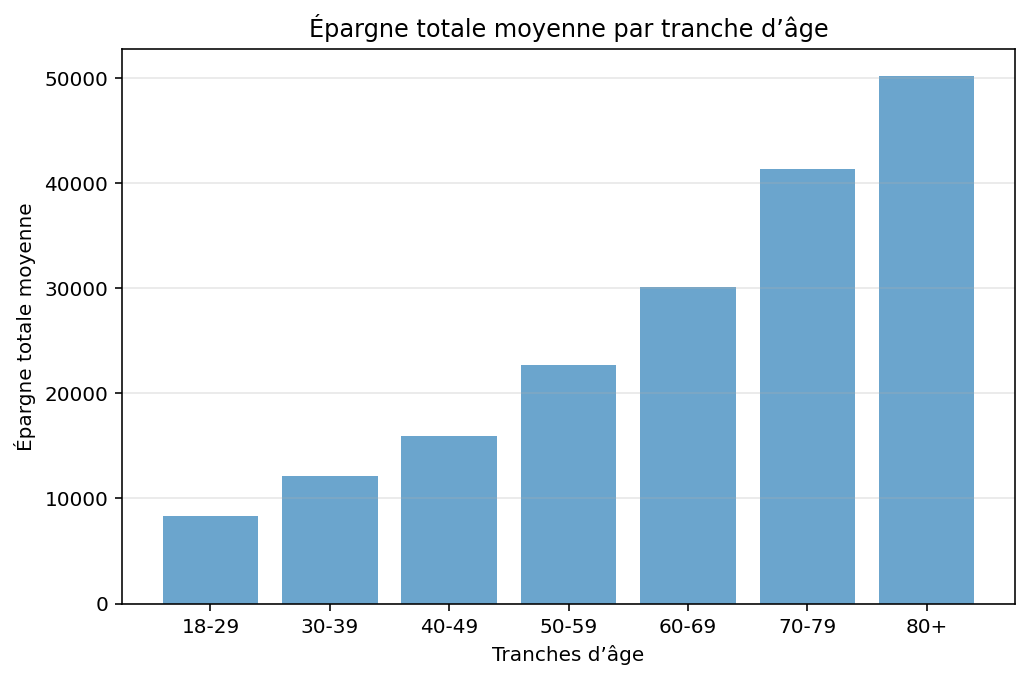
\includegraphics[width=0.5\textwidth]{images/py/epargneTotal_age.png}
    \caption{Histogramme de l'épargne totale selon l'âge}
\end{figure}

On observe une tendance claire : plus l'âge augmente, plus la moyenne d'épargne totale croît.  
Cela suggère un effet d'accumulation patrimoniale au fil du temps.

\subsubsection*{2. Histogramme de l'épargne financière par rapport à l'âge}
\begin{figure}[!h]
    \centering
    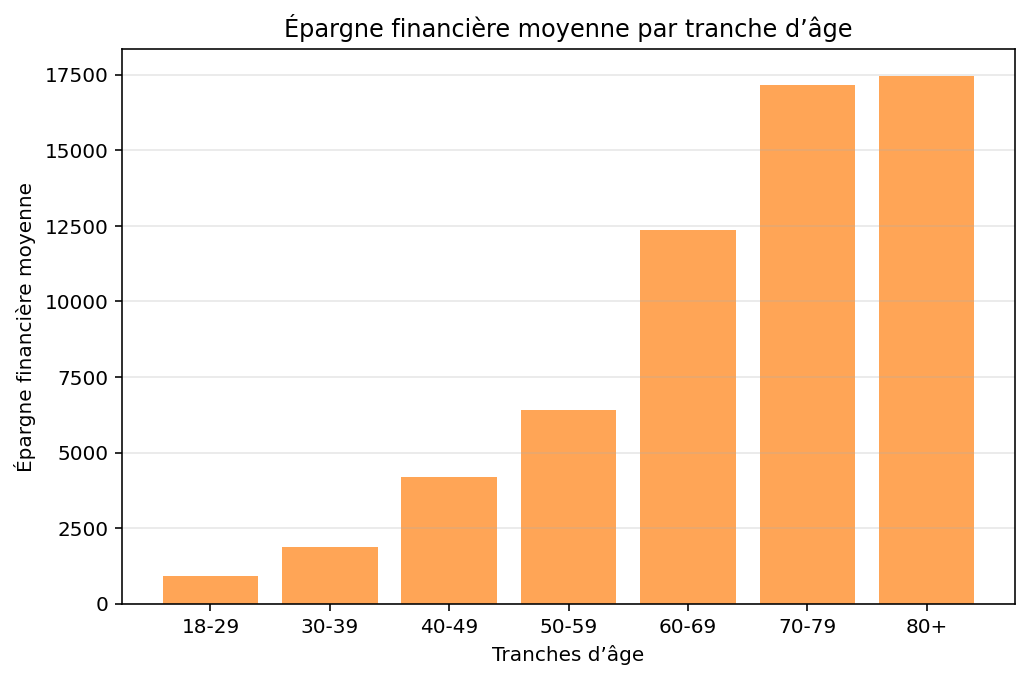
\includegraphics[width=0.5\textwidth]{images/py/eparge_fin_age.png}
    \caption{Histogramme de l'épargne financière selon l'âge}
\end{figure}

La même relation est visible que pour l'épargne totale : l'épargne financière progresse également avec l'âge, traduisant une capacité d'investissement plus forte chez les individus plus âgés.

\newpage\subsubsection*{3. Répartition de l'épargne totale par CSP}
\begin{figure}[h]
    \centering
    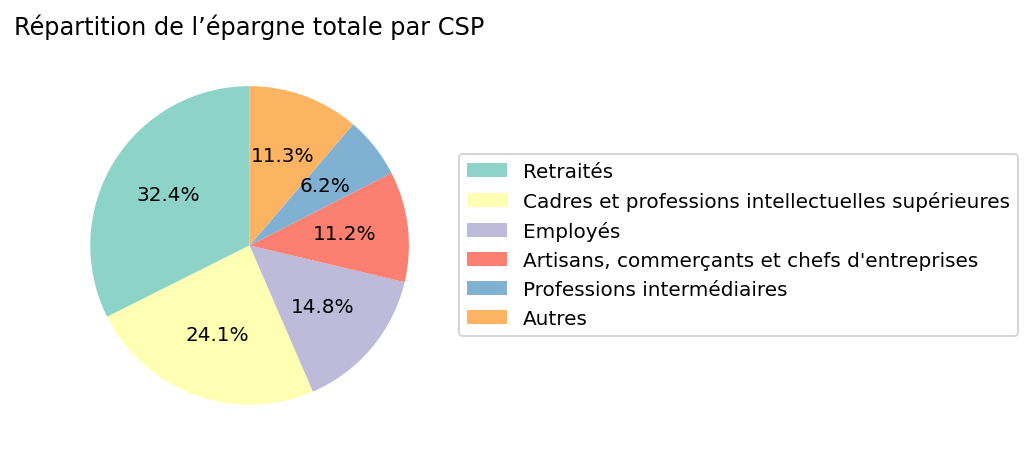
\includegraphics[width=0.6\textwidth]{images/py/CSP_epargne.png}
    \caption{Camembert de la répartition de l'épargne totale par CSP}
\end{figure}

La répartition montre que :  
- les \textbf{retraités} concentrent la part la plus importante (32,4\%),  
- suivis des \textbf{cadres et professions intellectuelles supérieures} (24,1\%),  
- puis des \textbf{employés} (14,8\%),  
- et des \textbf{artisans, commerçants et chefs d'entreprises} (11,2\%).  

Les autres catégories représentent des parts plus réduites.  
Cela confirme que les retraités, bénéficiant souvent de temps d’accumulation et de revenus stables, détiennent l'épargne la plus importante.

\subsubsection*{4. Répartition de l'épargne financière par CSP}
\begin{figure}[h]
    \centering
    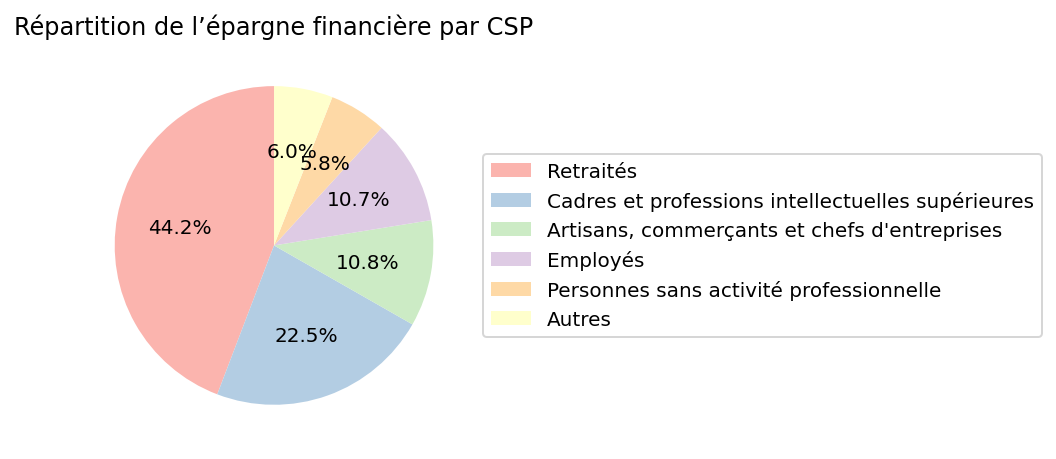
\includegraphics[width=0.6\textwidth]{images/py/csp_epargne_fin.png}
    \caption{Camembert de la répartition de l'épargne financière par CSP}
\end{figure}

La structure est encore plus marquée que pour l'épargne totale :  
- \textbf{44,2\% des retraités} concentrent à eux seuls près de la moitié de l'épargne financière,  
- suivis des \textbf{cadres et professions intellectuelles supérieures} (22,5\%).  

Les autres catégories (\textbf{artisans, employés, sans activité professionnelle}) se partagent le reste.  
Cette surreprésentation des retraités confirme leur rôle central dans l'épargne, probablement lié à une volonté de sécuriser le patrimoine.

\subsubsection*{5. Distribution des tranches d'épargne totale par marché}
\begin{figure}[!h]
    \centering
    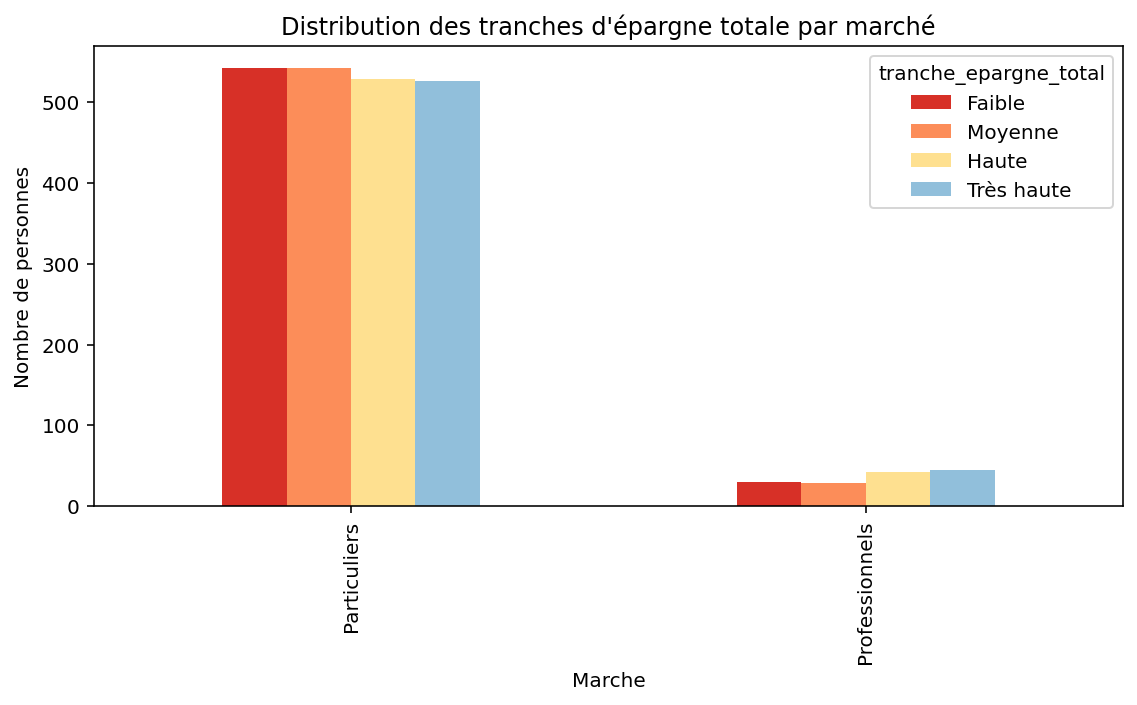
\includegraphics[width=0.7\textwidth]{images/py/epargne_total_marche.png}
    \caption{Histogramme des tranches d'épargne totale par marché}
\end{figure}

On constate une nette domination des particuliers, qui sont environ \textbf{cinq fois plus nombreux} que les professionnels.

\subsubsection*{6. Distribution des tranches d'épargne totale par type de client}
\begin{figure}[!h]
    \centering
    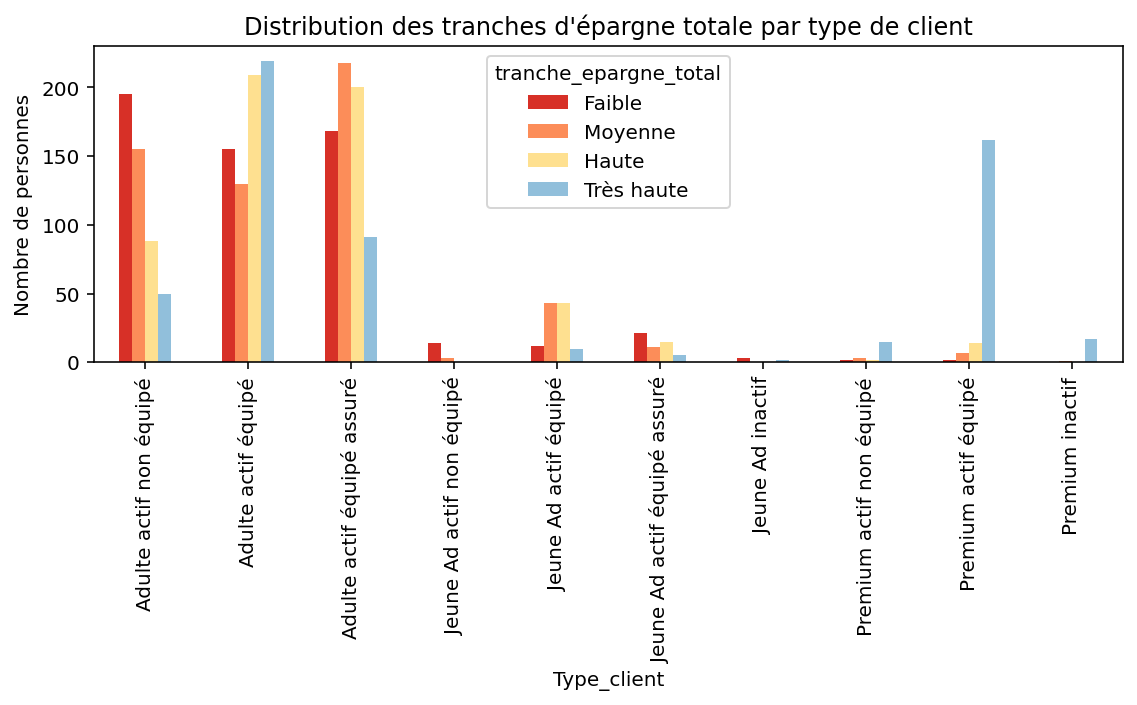
\includegraphics[width=0.7\textwidth]{images/py/epargne_total_typeClient.png}
    \caption{Histogramme des tranches d'épargne totale par type de client}
\end{figure}

L'analyse par type de client montre des contrastes importants :  
\begin{itemize}
    \item Les \textbf{adultes actifs non équipés} se concentrent surtout dans les tranches d’épargne faibles à moyennes
    \item Les \textbf{adultes actifs équipés}, en revanche, se distinguent par une forte présence dans les tranches hautes et très hautes, traduisant l'impact direct de l'équipement bancaire et assurantiel
    \item Les \textbf{adultes actifs équipés assurés} sont davantage répartis dans les niveaux faibles à moyens, ce qui suggère des profils plus hétérogènes
    \item Les \textbf{jeunes adultes actifs non équipés} disposent de très faibles niveaux d'épargne, quasiment inexistants dans les tranches supérieures
    \item Les \textbf{jeunes adultes actifs équipés (assurés ou non)} présentent une légère amélioration, mais restent globalement cantonnés aux tranches faibles à moyennes
    \item Les profils \textbf{premium} montrent un contraste très marqué : les \textbf{premium actifs équipés} et les \textbf{premium inactifs} concentrent quasi exclusivement leur épargne dans la tranche \textit{très haute}. Cela confirme leur statut patrimonial privilégié, fortement surreprésenté dans les épargnes les plus élevées
\end{itemize}

Ainsi, l'équipement bancaire et la catégorie premium apparaissent comme des facteurs discriminants majeurs pour expliquer le niveau d'épargne.

\subsection{Conclusion}

L'analyse exploratoire des données permet de dégager plusieurs enseignements clés :  

\begin{itemize}
    \item \textbf{Âge} : l'épargne (totale et financière) augmente régulièrement avec l'âge, confirmant un mécanisme d'accumulation patrimoniale.  
    \item \textbf{CSP} : les retraités dominent largement, suivis des cadres supérieurs, illustrant l'importance d'une carrière longue ou de revenus élevés dans la constitution d'un patrimoine.  
    \item \textbf{Marché} : les particuliers sont beaucoup plus nombreux, mais certains professionnels concentrent des montants d'épargne plus élevés.  
    \item \textbf{Type de client} : l'équipement joue un rôle central. Les adultes actifs équipés apparaissent comme les plus solides en termes d'épargne, tandis que les jeunes actifs non équipés restent vulnérables. Enfin, les profils premium sont quasi exclusivement positionnés dans les niveaux d'épargne les plus élevés, marquant une polarisation très forte.  
\end{itemize}

En résumé, l'âge, le statut socio-professionnel, l'équipement bancaire et l'appartenance à la catégorie premium constituent les principaux facteurs explicatifs de l'épargne.  
Ces résultats offrent une base précieuse pour la mise en place d'un modèle de prédiction visant à anticiper le potentiel d'épargne d'un individu en fonction de ses caractéristiques.